%!TEX root = ../main.tex
\chapter{Distribuzioni e spazi di Sobolev}
\LezioneV{25/03/21}
\section{Richiami su funzioni test e distribuzioni}

Sia $\displaystyle \Omega \subset \mathbb{R}^{n}$, $\displaystyle n\geqslant 1$.
\begin{definition}
    [Funzioni test]
    \begin{equation*}
        \mathcal{D}(\Omega) =\left\{\varphi :\Omega \rightarrow \mathbb{R} ,\ C^{\infty }(\Omega) \ \text{a supporto compatto}\right\}
    \end{equation*}
\end{definition}
Ricordiamo che il supporto di una funzione è la chiusura dell'insieme dove essa non si annulla.

L'insieme $\displaystyle \mathcal{D}(\Omega)$ è incluso in $\displaystyle L^{p}(\Omega) \ \forall p$, in particolare per $p=2$
\begin{equation*}
    \mathcal{D}(\Omega) \subset L^{2}(\Omega)
\end{equation*}
e l'inclusione è \textbf{densa}, ovvero per ogni elemento di $L^2 $ posso trovare una successione approssimante di funzioni in $\mathcal{D}$, più \emph{belle}:
\begin{equation*}
    \forall v\in L^{2}(\Omega) \ \exists \ (\varphi _{k})_{k} \subset \mathcal{D}(\Omega) \ \text{t.c.} \ \varphi _{n}\xrightarrow{L^{2}} v
\end{equation*}
o, alternativamente
\begin{equation*}
    \overline{\mathcal{D}(\Omega)}^{\Vert \cdotp \Vert _{L^{2}(\Omega)}} =L^{2}(\Omega)
\end{equation*}
\begin{definition}
    [Convergenza di funzioni test] Diciamo che
    \begin{equation*}
        \varphi _{n}\rightarrow \varphi \ \text{in} \ \mathcal{D}(\Omega)
    \end{equation*}
    Se:
    \begin{enumerate}
        \item $\displaystyle \exists K\subset \Omega$ compatto tale che $\text{supp} \varphi _{n} \subset K$ per ogni $n$.
        \item $\displaystyle \forall k\in \mathbb{N} ,\ \varphi ^{(k)}_{n}\rightarrow \varphi ^{(k)}$ uniformemente per $n\to \infty $.
    \end{enumerate}
\end{definition}
\begin{definition}
    [Distribuzioni] Sono gli elementi del \textbf{duale} delle funzioni test il duale, cioè in funzionali (ovvero che vanno in $\mathbb{R}$) lineari e continui partenti da $\mathcal{D}$:
    \begin{equation*}
        \mathcal{D} '(\Omega) =\left\{F:\mathcal{D}(\Omega)\rightarrow \mathbb{R} \ \text{lineari, continui}\right\}
    \end{equation*}
\end{definition}
Indichiamo \textit{l'azione di }$F$\textit{ su }$\displaystyle \varphi $:
\begin{equation*}
    F(\varphi) =F\varphi =\langle F,\varphi \rangle =_{\mathcal{D} '} \langle F,\varphi \rangle _{\mathcal{D}}
\end{equation*}
\begin{nb}
    La notazione
    \begin{equation*}
        \langle F,\varphi \rangle =\int _{\Omega } F\varphi
    \end{equation*}
    è formalmente errata, poiché col simbolo di integrale non si intende l'integrale che siamo soliti fare. Svolgiamo effettivamente un integrale se $\displaystyle u\in L^{2}(\Omega)$, in questo caso allora $\displaystyle Lu\in \mathcal{D} '(\Omega)$ e quando scriviamo
    \begin{equation*}
        \langle u,\varphi \rangle =\int _{\Omega } u(\x) \varphi (\x) \dxx
    \end{equation*}
    sottointendiamo in realtà
    \begin{equation*}
        \langle Lu,\varphi \rangle =\int _{\Omega } u(\x) \varphi (\x) \dxx
    \end{equation*}
\end{nb}
Esistono distribuzioni che non sono funzioni, come la $\displaystyle \delta _{n}$, ma nel caso in cui coincidano con delle funzioni il minimo sindacale è \
\begin{equation*}
    u\in L^{1}_{\text{loc}}(\Omega) \subset \mathcal{D} '(\Omega)
\end{equation*}
che è anche un'immersione continua.
\begin{definition}
    [Derivata debole o distribuzionale] Data $\displaystyle F\in \mathcal{D}'(\Omega)$ si definisce $\displaystyle \partial _{x_{i}} F\in \mathcal{D} '(\Omega)$
    \begin{equation*}
        \langle \partial _{x_{i}} F,\varphi \rangle =-\langle F,\partial _{x_{i}} \varphi \rangle
    \end{equation*}
    Se $\displaystyle F\in C^{1}(\overline{\Omega })$, quindi anche
    \begin{equation*}
        F\in C^{1}(\overline{\Omega }) \subset L^{2}(\Omega)\mathcal{\subset D} '(\Omega)
    \end{equation*}
    allora possiamo scrivere
    \begin{equation*}
        \langle F,\varphi \rangle =\int _{\Omega } F\varphi \dxx ,
    \end{equation*}
    e derivata debole e \textit{classica} \textbf{coincidono} (il $-$ salta fuori dall'integrazione per parti)
    \begin{align*}
        \langle \underbrace{\partial _{x_{i}} F}_{\text{classica}} ,\varphi \rangle & =\int _{\Omega } \partial _{x_{i}} F(\x) \varphi (\x) \dxx                                                                                          \\
                                                                                    & =\underbrace{\cancel{\int _{\partial \Omega } ...\varphi }}_{\varphi \text{ supp. comp.}} -\int _{\Omega } F(\x) \partial _{x_{i}} \varphi (\x)\dxx \\
                                                                                    & =-\langle F,\partial _{x_{i}} \varphi\rangle =\langle \underbrace{\partial _{x_{i}} F}_{\text{debole}} ,\varphi \rangle
    \end{align*}
\end{definition}
Estendiamo ora il nostro campo di lavoro alle \textbf{distribuzioni a valori vettoriali}, ovvero vettori di distribuzioni
\begin{equation*}
    \mathcal{D} '\left(\Omega ;\mathbb{R}^{n}\right) =[\mathcal{D} '(\Omega)]^{n} \ \ \ \ \mathbf{F} =(F_{1} ,..,F_{n}) \ \ \ \ \bm{\varphi } =(\varphi _{1} ,..,\varphi _{n})
\end{equation*}
L'azione di $\displaystyle \mathbf{F}$ su $\displaystyle \bm{\varphi }$ è
\begin{equation*}
    \langle \mathbf{F} ,\bm{\varphi } \rangle =\sum ^{n}_{i=1} \langle F_{i} ,\varphi _{i} \rangle
\end{equation*}
Da cui\footnote{Prestare attenzione all'utilizzo alternato, nei vari punti, di scalari o vettori.}:
\begin{itemize}
    \item il gradiente diventa divergenza

          \begin{equation*}
              \langle \nabla F,\bm{\varphi } \rangle =\sum ^{n}_{i=1} \langle \partial _{x_{i}} F,\varphi _{i} \rangle =-\sum ^{n}_{i=1} \langle F,\partial _{x_{i}} \varphi _{i} \rangle =-\langle F ,\sum ^{n}_{i=1} \partial _{x_{i}} \varphi _{i} \rangle
          \end{equation*}

          cioè
          \begin{equation*}
              \boxed{\langle \nabla F,\bm{\varphi } \rangle =-\langle F,\mathrm{div}\bm{\varphi } \rangle }
          \end{equation*}
    \item Con passaggi analoghi
          \begin{equation*}
              \boxed{\langle \mathrm{div}\mathbf{F} ,\varphi \rangle =-\langle \mathbf{F} ,\nabla \varphi \rangle }
          \end{equation*}
    \item mettendo insieme i risultati, otteniamo che il laplaciano può spostarsi liberamente dall'altra parte senza cambio di segno

          \begin{equation*}
              \langle \Delta F,\varphi \rangle =\langle \mathrm{div}(\nabla F) ,\varphi \rangle =-\langle \nabla F,\nabla \varphi \rangle =\langle F,\mathrm{div}(\nabla \varphi) \rangle
          \end{equation*}

          cioè
          \begin{equation*}
              \boxed{\langle \Delta F ,\varphi \rangle =\langle F,\Delta \varphi \rangle }
          \end{equation*}
\end{itemize}
\section{Esercizio (controesempio derivata debole-classica)}
\label{sec:controesempio-derivata-debole-classica}

Svolgiamo ora un esercizio (in buona parte di Analisi 2) per dimostrare come derivata debole e derivata classica possano non coincidere. Sia
\begin{equation*}
    \x =(x_{1} ,x_{2} ,x_{3}) \in \mathbb{R}^{3} \ \ \Rightarrow \ \ | \x| =\sqrt{x^{2}_{1} +x^{2}_{2} +x^{2}_{3}}
\end{equation*}
Sia
\begin{equation*}
    u(\x) =\frac{1}{| \x| } ,\ \x \neq \zer
\end{equation*}
Vogliamo trovare $\displaystyle \Delta u$.

\subsection{Derivata classica}

Osserviamo inanzitutto
\begin{equation*}
    \partial _{x_{i}}| \x| =\frac{2x_{i}}{2\sqrt{x_{1}^{2} +x_{2}^{2} +x_{3}^{2}}} =\frac{x_{i}}{|\x| } \ \ \Rightarrow \ \ \nabla | \x| =\frac{\x}{| \x| }
\end{equation*}
E per la regola della funzione composta
\begin{equation}
    \nabla f(| \x|) =f'(| \x|) \nabla | \x| =f'(| \x|)\frac{\x}{| \x| }
    \label{eq:chain-rule-composta}
\end{equation}
Allora possiamo calcolare $\displaystyle \Delta u$ usando \eqref{eq:chain-rule-composta}:
\begin{equation*}
    \Delta u(\x) =\Delta \left(\frac{1}{| \x| }\right) =\mathrm{div}\left(\nabla \left(\frac{1}{| \x| }\right)\right) =\mathrm{div}\left(-\frac{1}{| \x| ^{2}}\frac{\x}{| \x| }\right) =-\mathrm{div}\left(\frac{\x}{| \x| ^{3}}\right)
\end{equation*}
Usiamo ora l'identità di Leibniz
\begin{equation*}
    \mathrm{div}(g\mathbf{F}) =\nabla g\cdotp \mathbf{F} +g\mathrm{div}\mathbf{F} \ \ \text{con} \ g=\frac{1}{| \x| ^{3}} \ \text{e} \ \mathbf{F} =\x
\end{equation*}
\begin{equation*}
    -\mathrm{div}\left(\frac{\x}{| \x| ^{3}}\right) =-\left(\nabla \left(\frac{1}{| \x| ^{3}}\right) \cdotp \x +\frac{1}{| \x| ^{3}}\underbrace{\mathrm{div}\x}_{=3}\right) =-\left(-\frac{3}{| \x| ^{4}}\frac{\x}{| \x| } \cdotp \x +\frac{1}{| \x| ^{3}} 3\right)
\end{equation*}
e troviamo
\begin{equation*}
    \Delta u(\x) =-\left(-\frac{3}{| \x| ^{3}} +\frac{3}{| \x| ^{3}}\right) =0
\end{equation*}
Quindi $u$ è armonica in $\displaystyle \mathbb{R}^{3} \backslash \{\zer\}$.

\subsection{Derivata distribuzionale}

Per poter fare la derivata distribuzionale dobbiamo prima chiederci
\begin{equation*}
    u\in L^{1}_{\text{loc}}\left(\mathbb{R}^{3}\right) ?
\end{equation*}
L'unico problema della funzione è, ovviamente, nell'origine. Se l'integrale su una palla unitaria centrata nell'origine convergerà la condizione sarà soddisfatta.
\begin{equation*}
    \int _{B_{1}(\zer)}\frac{1}{| \x| } \dxx =\int ^{1}_{0}\left(\int _{\partial B_{r}}\frac{1}{| \x| } \dsig \right) \dr=\int ^{1}_{0}\frac{1}{r} 4\pi r^{2} \dr< +\infty
\end{equation*}
Abbiamo utilizzato una formula di coarea (o integrazione per bucce)
\begin{equation*}
    \int _{B_{R}} f\dxx =\int ^{R}_{0}\left(\int _{\partial B_{r}} f\dsig \right) \dr
\end{equation*}
Quindi $\displaystyle u\in L_{\text{loc}}^{1}$ ed è pertanto associata a una distribuzione $\displaystyle u\in \mathcal{D} '\left(\mathbb{R}^{3}\right)$.

Per calcolare $\displaystyle \Delta u$ in $\displaystyle \mathcal{D} '\left(\mathbb{R}^{3}\right)$ prendiamo una funzione test $\displaystyle \varphi \in \mathcal{D}\left(\mathbb{R}^{3}\right)$
\begin{equation*}
    \langle \Delta u,\varphi \rangle =\langle u,\Delta \varphi \rangle \underbrace{=}_{u\in L^{1}_{\text{loc}}}\int _{\mathbb{R}^{3}}\frac{1}{| \x| } \Delta \varphi (\x) \dxx \
\end{equation*}
Quest'integrale presenta due problemi
\begin{enumerate}
    \item Il dominio è \textbf{illimitato}: in realtà dato che
          \begin{equation*}
              \text{supp} \varphi \subset B_{R}(\zer)
          \end{equation*}

          poiché $\displaystyle \varphi $ è a supporto compatto mi basterà limitare il dominio di integrazione a tale palla
    \item Ho una \textbf{singolarità} nell'origine: aggiriamo il problema integrando su un dominio $\displaystyle B_{R}(\zer) \backslash B_{\varepsilon }(\zer)$ e facendo il limite per $\displaystyle \varepsilon \rightarrow 0$

          \begin{figure}[htpb]
              \centering
              \tikzset{every picture/.style={line width=0.75pt}} %set default line width to 0.75pt        

              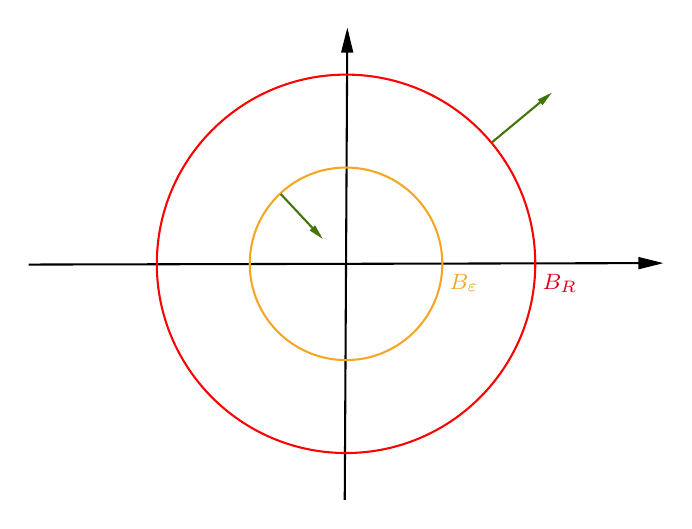
\begin{tikzpicture}[x=0.75pt,y=0.75pt,yscale=-1,xscale=1]
                  %uncomment if require: \path (0,251); %set diagram left start at 0, and has height of 251

                  %Straight Lines [id:da018527204913219464] 
                  \draw    (74.4,123.02) -- (378.17,122.31) ;
                  \draw [shift={(380.17,122.31)}, rotate = 539.87] [fill={rgb, 255:red, 0; green, 0; blue, 0 }  ][line width=0.08]  [draw opacity=0] (12,-3) -- (0,0) -- (12,3) -- cycle    ;
                  %Straight Lines [id:da8598068958336733] 
                  \draw    (226.66,236.38) -- (227.9,10.94) ;
                  \draw [shift={(227.91,8.94)}, rotate = 450.32] [fill={rgb, 255:red, 0; green, 0; blue, 0 }  ][line width=0.08]  [draw opacity=0] (12,-3) -- (0,0) -- (12,3) -- cycle    ;
                  %Shape: Ellipse [id:dp6985117247796604] 
                  \draw  [color={rgb, 255:red, 245; green, 166; blue, 35 }  ,draw opacity=1 ] (180.89,122.66) .. controls (180.89,97.04) and (201.66,76.27) .. (227.28,76.27) .. controls (252.91,76.27) and (273.68,97.04) .. (273.68,122.66) .. controls (273.68,148.28) and (252.91,169.05) .. (227.28,169.05) .. controls (201.66,169.05) and (180.89,148.28) .. (180.89,122.66) -- cycle ;
                  %Straight Lines [id:da5357301688162748] 
                  \draw [color={rgb, 255:red, 65; green, 117; blue, 5 }  ,draw opacity=1 ]   (195.8,89) -- (214.64,109.14) ;
                  \draw [shift={(216,110.6)}, rotate = 226.91] [fill={rgb, 255:red, 65; green, 117; blue, 5 }  ,fill opacity=1 ][line width=0.08]  [draw opacity=0] (7.2,-1.8) -- (0,0) -- (7.2,1.8) -- cycle    ;
                  %Straight Lines [id:da996019003751347] 
                  \draw [color={rgb, 255:red, 65; green, 117; blue, 5 }  ,draw opacity=1 ]   (297.75,64) -- (324.79,41.56) ;
                  \draw [shift={(326.33,40.28)}, rotate = 500.31] [fill={rgb, 255:red, 65; green, 117; blue, 5 }  ,fill opacity=1 ][line width=0.08]  [draw opacity=0] (7.2,-1.8) -- (0,0) -- (7.2,1.8) -- cycle    ;
                  %Shape: Ellipse [id:dp7419991498839904] 
                  \draw  [color={rgb, 255:red, 255; green, 0; blue, 0 }  ,draw opacity=1 ] (136.12,122.66) .. controls (136.12,72.31) and (176.94,31.5) .. (227.28,31.5) .. controls (277.63,31.5) and (318.45,72.31) .. (318.45,122.66) .. controls (318.45,173.01) and (277.63,213.82) .. (227.28,213.82) .. controls (176.94,213.82) and (136.12,173.01) .. (136.12,122.66) -- cycle ;

                  % Text Node
                  \draw (320.45,126.06) node [anchor=north west][inner sep=0.75pt]  [font=\footnotesize,color={rgb, 255:red, 208; green, 2; blue, 27 }  ,opacity=1 ]  {$B_{R}$};
                  % Text Node
                  \draw (275.68,126.06) node [anchor=north west][inner sep=0.75pt]  [font=\footnotesize,color={rgb, 255:red, 245; green, 166; blue, 35 }  ,opacity=1 ]  {$B_{\varepsilon }$};
                  % Text Node
                  \draw (328.93,39.81) node [anchor=north west][inner sep=0.75pt]  [font=\normalsize,color={rgb, 255:red, 65; green, 117; blue, 5 }  ,opacity=1 ]  {$\nuu$};
                  % Text Node
                  \draw (191.73,99.01) node [anchor=north west][inner sep=0.75pt]  [font=\normalsize,color={rgb, 255:red, 65; green, 117; blue, 5 }  ,opacity=1 ]  {$\nuu$};


              \end{tikzpicture}
          \end{figure}
          \FloatBarrier
          \begin{equation}
              \int _{\mathbb{R}^{3}}\frac{1}{| \x| } \Delta \varphi (\x) \dxx \ =\lim _{\varepsilon \rightarrow 0}\int _{B_{R} \backslash B_{\varepsilon }}\frac{1}{| \x| } \Delta \varphi (\x) \dxx
              \label{eq:esempio-derivata-limite}
          \end{equation}
\end{enumerate}

Ora $\displaystyle \frac{1}{| \x| }$ è $\displaystyle C^{\infty }$ nel dominio di integrazione e posso applicare la formula di integrazione per parti che ricordiamo qua sotto
\begin{equation*}
    \int _{\Omega } u\Delta v=\int _{\partial \Omega } u\partial _{\nuu} v-\int _{\Omega } \nabla u\cdotp \nabla v=\int _{\partial \Omega } u\partial _{\bm{\nu }} v-\int _{\partial \Omega } v\partial _{\bm{\nu }} u+\int _{\Omega } v\Delta u
\end{equation*}
con
\begin{equation*}
    u=\frac{1}{| \x| } ,\ v=\varphi (\x) ,\ \partial \Omega =\partial B_{R} \cup \partial B_{\varepsilon }
\end{equation*}
La normale $\displaystyle \bm{\nu }$ sarà diretta verso l'esterno o l'interno a seconda che mi trovi rispettivamente su $\displaystyle \partial B_{R}$ o $\displaystyle \partial B\varepsilon $.

Osserviamo inoltre che essendo $\displaystyle \varphi \in \mathcal{D}\left(\mathbb{R}^{3}\right)$
\begin{equation*}
    \partial _{\bm{\nu }} \varphi \equiv \varphi \equiv 0\ \text{su} \ \partial B_{R}
\end{equation*}
Pertanto gli integrali sul bordo esterno si semplificano subito
\begin{equation*}
    \cancel{\textcolor[rgb]{0.25,0.46,0.02}{\int _{\partial B_{R}}}} \ \ \cancel{\textcolor[rgb]{0.29,0.56,0.89}{\int _{\partial B_{R}}}}
\end{equation*}
Applicando il tutto a \eqref{eq:esempio-derivata-limite} otteniamo

\begin{equation}
    \lim _{\varepsilon \rightarrow 0}\left[\textcolor[rgb]{0.25,0.46,0.02}{\int _{\partial B_{\varepsilon }}\frac{1}{| \x| } \partial _{\nuu} \varphi (\x) \dsig } -\textcolor[rgb]{0.29,0.56,0.89}{\int _{\partial B_{\varepsilon }} \varphi (\x) \partial _{\nuu}\left(\frac{1}{| \x| }\right) \dsig } +\textcolor[rgb]{0.82,0.01,0.11}{\int _{B_{R} \backslash B_{\varepsilon }} \varphi (\x) \Delta \left(\frac{1}{| \x| }\right) \dxx}\right]
    \label{eq:esempio-derivata-limite-2}
\end{equation}
Di questi termini
\begin{itemize}
    \item essendo $\displaystyle \Delta u=0$ il laplaciano classico in $\displaystyle B_{R} \backslash B_{\varepsilon }$:
          \begin{equation*}
              \textcolor[rgb]{0.82,0.01,0.11}{\int _{B_{R} \backslash B_{\varepsilon }} \varphi (\x) \Delta \left(\frac{1}{| \x| }\right) \dxx} =0
          \end{equation*}
    \item  $\displaystyle \partial _{\nuu} \varphi =\nabla \varphi \cdotp \nuu$, dove $\displaystyle \nuu =-\frac{\x}{| \x| }$ essendo orientata in dentro
          \begin{equation*}
              \textcolor[rgb]{0.25,0.46,0.02}{\int _{\partial B_{\varepsilon }}\frac{1}{| \x| } \partial _{\nuu} \varphi (\x) \dsig } =\textcolor[rgb]{0.25,0.46,0.02}{-\int _{\partial B_{\varepsilon }}\frac{1}{| \x| } \nabla \varphi (\x) \cdotp \frac{\x}{| \x| } \dsig }
          \end{equation*}
    \item $\displaystyle \partial _{\nuu}\left(\frac{1}{| \x| }\right) =\nabla \left(\frac{1}{| \x| }\right) \cdotp \nuu$, con $\displaystyle \nuu$ identica a prima
          \begin{equation*}
              \textcolor[rgb]{0.29,0.56,0.89}{\int _{\partial B_{\varepsilon }} \varphi (\x) \partial_{\nuu}\left(\frac{1}{| \x| }\right) \dsig } =-\int _{\partial B_{\varepsilon }} \varphi (\x)\left(-\frac{\x}{| \x| ^{3}}\right) \cdotp \left(-\frac{\x}{| \x| }\right) \dsig =\textcolor[rgb]{0.29,0.56,0.89}{-\int _{\partial B_{\varepsilon }} \varphi (\x)\frac{1}{| \x| ^{2}} \dsig }
          \end{equation*}
\end{itemize}

Inoltre su $\displaystyle \partial B_{\varepsilon }$: $\displaystyle | \x| =\varepsilon $. Possiamo riscrivere \eqref{eq:esempio-derivata-limite-2}:
\begin{equation*}
    \lim _{\varepsilon \rightarrow 0}\left[\textcolor[rgb]{0.25,0.46,0.02}{-\frac{1}{\varepsilon ^{2}}\int _{\partial B_{\varepsilon }} \nabla \varphi (\x) \cdotp \x \dsig }\textcolor[rgb]{0.29,0.56,0.89}{-\frac{1}{\varepsilon ^{2}}\int _{\partial B_{\varepsilon }} \varphi (\x) \dsig }\right]
\end{equation*}
Se entrambi i termini tendono a $0$ allora la mia derivata distribuzionale coinciderà con quella classica. Esaminiamoli separatamente:
\begin{itemize}
    \item primo termine

          \begin{equation*}
              \left| \textcolor[rgb]{0.25,0.46,0.02}{-\frac{1}{\varepsilon ^{2}}\int _{\partial B_{\varepsilon }} \nabla \varphi (\x) \cdotp \x \dsig }\right| \leqslant \frac{1}{\varepsilon ^{2}}\int _{\partial B_{\varepsilon }}| \nabla \varphi (\x)| \cdotp | \x| \dsig
          \end{equation*}

          $\displaystyle | \nabla \varphi | \leqslant c$ essendo $\displaystyle \varphi $ una funzione test e su $\displaystyle \partial B_{\varepsilon }$: $\displaystyle | \x| =\varepsilon $
          \begin{equation*}
              \frac{1}{\varepsilon ^{2}}\int _{\partial B_{\varepsilon }}\underbrace{| \nabla \varphi (\x)| }_{\leqslant c} \cdotp \underbrace{| \x| }_{=\varepsilon } \dsig \leqslant \frac{c}{\varepsilon }\underbrace{\int _{\partial B_{\varepsilon }} \dsig }_{4\pi \varepsilon ^{2}} =\frac{c}{\varepsilon } 4\pi \varepsilon ^{2}\textcolor[rgb]{0.25,0.46,0.02}{\rightarrow 0}
          \end{equation*}
    \item secondo termine

          Posso usare il teorema della media integrale essendo $\displaystyle \varphi $ continua

          \begin{equation*}
              \textcolor[rgb]{0.29,0.56,0.89}{-\frac{1}{\varepsilon ^{2}}\int _{\partial B_{\varepsilon }} \varphi (\x) \dsig } =-4\pi \frac{1}{4\pi \varepsilon ^{2}}\int _{\partial B_{\varepsilon }} \varphi (\x) \dsig =-4\pi \underbrace{\frac{1}{| \partial B_{\varepsilon }| }\int _{\partial B_{\varepsilon }} \varphi (\x) \dsig }_{=\varphi (\x_{\varepsilon })\xrightarrow{\varepsilon \rightarrow 0} \varphi (\zer)}\rightarrow -4\pi \varphi (\zer)
          \end{equation*}

          per un certo $\displaystyle \x_{\varepsilon } \in \partial B_{\varepsilon }$.
\end{itemize}

Riassumendo\footnote{il simbolo $\displaystyle \delta _{3}$ non indica la Delta centrata in $3$, ma la delta tridimensionale centrata in $0$.}
\begin{equation*}
    \langle \Delta u,\varphi \rangle =-4\pi \varphi (\zer) =-4\pi \langle \delta _{3} ,\varphi \rangle \ \ \Rightarrow \ \ -\Delta \left(\frac{1}{4\pi }\frac{1}{| \x| }\right) =\delta _{3} \ \text{in} \ \mathcal{D} '\left(\mathbb{R}^{3}\right)
\end{equation*}
La derivata classica e debole non coincidono.

\section{Spazi di Sobolev}
\LezioneV{01/04/2021}

Gli spazi di Sobolev sono ``spazi di funzioni $L^{p}$ aventi derivate $L^{p}$''. Lavoreremo con due spazi di Sobolev, il primo sarà $H^{1}$ e il secondo $H^{1}_{0} \subseteq H^{1}$.

Consideriamo $\Omega \subset \mathbb{R}^{n}$ dominio (cioè aperto connesso)\footnote{di solito saranno limitati, ma possiamo tranquillamente immaginare che siano tutto $\mathbb{R}^{n}$.}.
\begin{definition}
    \begin{equation*}
        H^{1}(\Omega) =\left\{v\in L^{2}(\Omega) :\nabla v\in L^{2}\left(\Omega ;\mathbb{R}^{n}\right)\right\}
    \end{equation*}
    $\nabla v$ è inteso \textbf{nel senso delle distribuzioni}.
\end{definition}
Questo spazio è dotato di prodotto scalare
\begin{equation*}
    (u,v)_{H^{1}(\Omega)} =(\nabla u,\nabla v)_{L^{2}(\Omega)} +(u,v)_{L^{2}(\Omega)} =\int _{\Omega }[ \nabla u(\x) \cdotp \nabla v(\x) +u(\x) v(\x)] \dxx
\end{equation*}
In particolare vale il seguente risultato delle norme
\begin{equation*}
    \Vert u\Vert ^{2}_{H^{1}(\Omega)} =\Vert u\Vert ^{2}_{L^{2}} +\Vert \nabla u\Vert ^{2}_{L^{2}} \geqslant \begin{cases}
        \Vert u\Vert ^{2}_{L^{2}} \\
        \Vert \nabla u\Vert ^{2}_{L^{2}}
    \end{cases}
\end{equation*}
misurando le norme in $H^{1}$ stiamo contemporaneamente controllando sia la norma della funzione, che delle sue derivate parziali.
\begin{theorem}
    [Microteorema]
    Valgono i seguenti enunciati:
    \begin{enumerate}
        \item $H^{1}(\Omega)$ è uno spazio di Hilbert\footnote{si può dimostrare verificando tutte le proprietà di uno spazio di Hilbert, sfruttando il fatto che $L^{2}$ è di Hilbert.},
        \item $H^{1}(\Omega) \hookrightarrow L^{2}(\Omega)$, $H^{1}$ si immerge in $L^{2}$ con continuità, cioè come abbiamo appena scritto che la norma di $H^{1}$ è più \textit{forte} della norma di $L^{2}$,
        \item $\nabla :H^{1}(\Omega)\rightarrow L^{2}\left(\Omega ;\mathbb{R}^{n}\right)$ è lineare e continuo.
    \end{enumerate}
\end{theorem}

Notiamo che $H^{1}$ è, oltre che un sottoinsieme, anche un \textbf{sottospazio chiuso} di $L^{2}$.

In generale, anche se non li useremo, si definiscono gli spazi
\begin{equation*}
    H^{k}(\Omega) =\left\{v\in L^{2} :D^{\bm{\alpha}} v\in L^{2} ,\ \forall | \bm{\alpha}| \leqslant k\right\}
\end{equation*}
La notazione $D^{\bm{\alpha}}$ significa che intendiamo le derivate prime, seconde, terze, ecc, fino alla $n$-esima derivazione
\begin{equation*}
    \bm{\alpha} =(\alpha _{1} ,\dotsc ,\alpha _{n}) \ \ \Rightarrow \ \ D^{\bm{\alpha}} v=\partial ^{\alpha _{1}}_{x_{1}} \partial ^{\alpha _{2}}_{x_{2}} \dotsc \partial ^{\alpha _{n}}_{x_{n}} v
\end{equation*}
Useremo solitamente solo $H^{1} ,H^{2}$.

Ancora più in generale gli \textbf{spazi di Sobolev} sono
\begin{equation*}
    W^{k,p}(\Omega) =\left\{v\in L^{p}(\Omega) :D^{\bm{\alpha}} v\in L^{p} ,\ \forall | \bm{\alpha}| \leqslant k\right\}
\end{equation*}
Facciamo un po' la conoscenza di questi spazi:
\begin{gather*}
    \mathcal{D}(\Omega) \subset H^{1}(\Omega) ,\\
    C^{1}(\overline{\Omega }) \subset H^{1}(\Omega) \ \text{se} \ | \Omega | < +\infty ,\ \text{non in generale perché devono stare in} \ L^{2}
\end{gather*}
$H^{1}(\Omega)$ può contenere anche delle funzioni discontinue.

\textit{Esempio.}
\begin{equation*}
    B_{1}(\zer) \subset \mathbb{R}^{3} ,\ \ u(\x) =| \x| ^{-a} \ \ (a >0)
\end{equation*}
È una funzione non definita in $\zer$, per quali valori di $a$ si ha che $u\in H^{1}(B_{1})$?
\begin{enumerate}
    \item $u\overset{?}{\in } L^{2}(B_{1}) :$
          \begin{align*}
              \int _{B_{1}} u^{2}(\x) \dxx & =\int _{B_{1}}| \x| ^{-2a} \dxx =\int ^{1}_{0}\left[\int _{\partial B_{r}}| \x| ^{-2a} \dsig \right] \dr \\
                                           & =\int ^{1}_{0}| r| ^{-2a} \cdotp 4\pi r^{2} \dr=4\pi \int ^{1}_{0} r^{2-2a} \dr                          \\
                                           & < +\infty \ \ \Leftrightarrow \ \ 2-2a >-1\ \ \Leftrightarrow \ \ a< \frac{3}{2}
          \end{align*}
    \item Calcoliamo il gradiente
          \begin{equation*}
              \nabla u(\x) =-a| \x| ^{-a-1} \cdotp \frac{\x}{| \x| } =-a| \x| ^{-a-2}\x
          \end{equation*}

          per quali valori sta in $L^{2}$? $\nabla u\overset{?}{\in } L^{2}(B_{1}) :$
          \begin{align*}
              \int _{B_{1}} a^{2}| \x| ^{-2a-4+2} \dxx & =\int ^{1}_{0}\left[ a^{2} r^{-2a-2} \cdotp 4\pi r^{2}\right] \dr               \\
                                                       & =a^{2} 4\pi \int ^{1}_{0} r^{-2a} \dr                                           \\
                                                       & < +\infty \ \ \Leftrightarrow \ \ -2a >-1\ \ \Leftrightarrow \ \ a< \frac{1}{2}
          \end{align*}
\end{enumerate}

mettendo assieme
\begin{equation*}
    u\in H^{1}(B_{1}) \ \ \Leftrightarrow \ \ \left\{a >0\ \ \land \ \ a< \frac{3}{2} \ \ \land \ \ a< \frac{1}{2}\right\} \ \ \Leftrightarrow \ \ 0< a< \frac{1}{2}
\end{equation*}
\textbf{Verzini ci ha burlati}, ha calcolato il \textbf{gradiente classico}, invece andava calcolato come
\begin{equation*}
    \langle \nabla u,\bm{\varphi} \rangle =-\langle u,\mathrm{div}\bm{\varphi} \rangle
\end{equation*}
a questo punto $u\in L^{1}_{\mathrm{loc}}$, scrivo l'integrale, tolgo la palla nell'origine, ecc. come l'altra volta. Facendo i conti si trova che era sufficiente che $a$ fosse minore di $\frac{3}{2}$.

L'obiettivo finale sarà risolvere
\begin{equation*}
    \begin{cases}
        -\Delta u=f(\x) & \x \in \Omega          \\
        u=0             & \x \in \partial \Omega
    \end{cases}
\end{equation*}
\begin{oss}
    Come interpretare le condizioni al contorno? Dato che le funzioni di $H^{1}$ sono \textit{quasi} funzioni di $L^{2}$, ci dobbiamo ricordare che le funzioni non erano proprio funzioni, ma \textbf{classi di equivalenza di funzioni}. Cioè due funzioni sono equivalenti se sono uguali a meno di un insieme di misura nulla e spesso
    \begin{equation*}
        | \partial \Omega | _{n\text{-dimensionale}} =0
    \end{equation*}
    Che senso ha dire che $u=0$ su un insieme di misura nulla? Lo scopriremo più avanti (Teoria delle Tracce: sotto ipotesi su $\Omega $, bordo lipschitziano, se $u\in H^{1}(\Omega)$ allora $u$ sul bordo di $\Omega $ ha senso. La \textit{traccia} di $u$ è la restrizione di $u$ al bordo $u_{|\partial \Omega }$).
\end{oss}
Noi tratteremo $2$ situazioni facili:
\begin{itemize}
    \item $n=1$, $\Omega =(a,b)$. Daremo un senso alla traccia, cioè quanto vale $u(a) ,u(b)$.
    \item $n=n,\Omega =\Omega $, ma $u_{|\partial \Omega } =0$. Non discuteremo se $u=g$.
\end{itemize}

$H^{1}$ è più piccolo e gode di più proprietà: in dimensione $n=1$ le funzioni di $H^{1}$ sono continue fino al bordo\footnote{o meglio, ammettono un \textit{rappresentante} continuo fino al bordo.}. Questo fatto non è vero in dimensione più alta, abbiamo visto un esempio.
\begin{theorem}
    [Microteorema] In dimensione $n=1$, $u\in L^{2}(a,b)$. Allora
    \begin{equation*}
        u\in H^{1}(a,b) \ \ \Leftrightarrow \ \ \begin{cases}
            u\in C([ a,b]) ,            & \text{(cioè esiste un rappresentate continuo)} \\
            \begin{array}{l}
                \exists \ w\in L^{2}(a,b) \ \text{t.c.} \\
                u(x) -u(y) =\int ^{x}_{y} w(s) \ds
            \end{array} & \begin{array}{l}
                \forall x,y\in [ a,b] \\
                \text{(essenzialmente il TFCI)}
            \end{array}
        \end{cases}
    \end{equation*}
    Inoltre
    \begin{equation*}
        u'=w
    \end{equation*}
    sia nel senso $\mathcal{D} '$ che quasi ovunque, derivata debole e classica coincidono quasi ovunque.
\end{theorem}
Per esempio Heaviside, che in effetti non sta in $H^{1}$, non ha derivata classica e debole coincidenti.

Il punto del teorema che ci interessa è dire che se $u\in H^{1}$ allora è continua fino al bordo e possiamo dare un senso ai valori che assume in $a,b$.
\begin{dimostrazione}
    $(\Rightarrow)$ $u\in H^{1}(a,b)$ allora la sua derivata debole $u'\in L^{2}(a,b)$.

    Definisco
    \begin{equation*}
        v(x) =\int ^{x}_{a} u'(s) \ds
    \end{equation*}
    Attenzione: posso dire che $v(x) =u(x) -u(a)$? Non per forza, per applicare il TFCI l'integranda $u'$ deve essere continua, ma sta solo in $L^{2}$. Dimostreremo che sarà vero.

    $v$ è continua fino al bordo:
    \begin{align*}
        x_{n}\rightarrow x\ \ \Rightarrow \ \ | v(x_{n}) -v(x)| & =\left| \int ^{x_{n}}_{x} 1\cdot u'(s) \ds\right|                                                                                          &                                 \\
                                                                & \leqslant | x_{n} -x| ^{1/2}\left(\int ^{x_{n}}_{x}(u')^{2}\right)^{1/2}                                                                   & \text{(Cauchy-Schwarz)}         \\
                                                                & \leqslant \underbrace{| x_{n} -x| ^{1/2}}_{\rightarrow 0}\underbrace{\left(\int ^{b}_{a}(u')^{2}\right)^{1/2}}_{\leqslant C,\ u'\in L^{2}} & \text{(l'integrale è positivo)} \\
                                                                & \rightarrow 0                                                                                                                              &
    \end{align*}
    $v$ continua implica che è funzione di $L^{1}_{\mathrm{loc}}$, quindi associata a una distribuzione.

    Calcolo $v'$ (in $\mathcal{D} '(a,b)$). $\forall \varphi \in \mathcal{D}(a,b)$
    \begin{align*}
        \langle v',\varphi \rangle & =-\langle v,\varphi '\rangle                                                             \\
                                   & =-\int ^{b}_{a} v(x) \varphi '(x) \dx                                                    \\
                                   & =-\int ^{b}_{a}\underbrace{\left[\int ^{x}_{a} u'(s) \ds\right]}_{v(x)} \varphi '(x) \dx \\
                                   & =-\iint _{T}[ u'(s) \varphi '(x)] \ds\dx=(*)
    \end{align*}

    \begin{figure}[H]
        \centering
        \tikzset{every picture/.style={line width=0.75pt}} %set default line width to 0.75pt        

        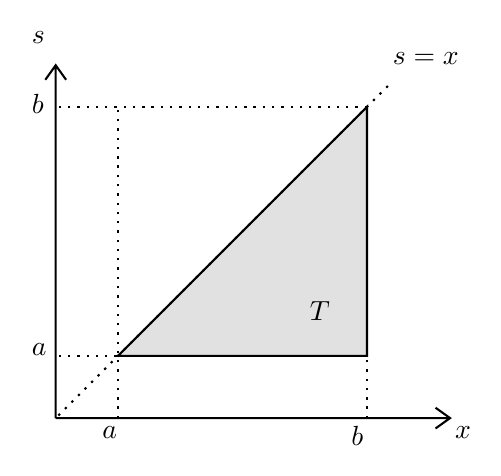
\begin{tikzpicture}[x=0.75pt,y=0.75pt,yscale=-1,xscale=1]
            %uncomment if require: \path (0,235); %set diagram left start at 0, and has height of 235

            %Shape: Axis 2D [id:dp784008935667821] 
            \draw  (210,200) -- (400,200)(210,30) -- (210,200) -- cycle (393,195) -- (400,200) -- (393,205) (205,37) -- (210,30) -- (215,37)  ;
            %Straight Lines [id:da7455693777283228] 
            \draw  [dash pattern={on 0.84pt off 2.51pt}]  (240,200) -- (240,50) ;
            %Straight Lines [id:da4914420152692185] 
            \draw  [dash pattern={on 0.84pt off 2.51pt}]  (360,200) -- (360,50) ;
            %Straight Lines [id:da009766020008167953] 
            \draw  [dash pattern={on 0.84pt off 2.51pt}]  (360,170) -- (210,170) ;
            %Straight Lines [id:da9309333949976712] 
            \draw  [dash pattern={on 0.84pt off 2.51pt}]  (360,50) -- (210,50) ;
            %Straight Lines [id:da2896330081060874] 
            \draw  [dash pattern={on 0.84pt off 2.51pt}]  (370,40) -- (210,200) ;
            %Shape: Polygon [id:ds48703033858893674] 
            \draw  [fill={rgb, 255:red, 155; green, 155; blue, 155 }  ,fill opacity=0.3 ] (360,50) -- (240,170) -- (360,170) -- cycle ;

            % Text Node
            \draw (371,22.4) node [anchor=north west][inner sep=0.75pt]    {$s=x$};
            % Text Node
            \draw (401,202.4) node [anchor=north west][inner sep=0.75pt]    {$x$};
            % Text Node
            \draw (197,12.4) node [anchor=north west][inner sep=0.75pt]    {$s$};
            % Text Node
            \draw (231,202.4) node [anchor=north west][inner sep=0.75pt]    {$a$};
            % Text Node
            \draw (351,202.4) node [anchor=north west][inner sep=0.75pt]    {$b$};
            % Text Node
            \draw (197,162.4) node [anchor=north west][inner sep=0.75pt]    {$a$};
            % Text Node
            \draw (197,42.4) node [anchor=north west][inner sep=0.75pt]    {$b$};
            % Text Node
            \draw (331,142.4) node [anchor=north west][inner sep=0.75pt]    {$T$};

        \end{tikzpicture}
    \end{figure}
    \FloatBarrier

    \begin{align*}
        (*) & =-\int ^{b}_{a}\left[\int ^{b}_{s} u'(s) \varphi '(x) \dx\right] \ds    &                            \\
            & =-\int ^{b}_{a} u'(s)\left[\int ^{b}_{s} \varphi '(x) \dx\right] \ds    &                            \\
            & =-\int ^{b}_{a} u'(s)\left[\cancel{\varphi (b)} -\varphi (s)\right] \ds &                            \\
            & =\int ^{b}_{a} u'(s) \varphi (s) \ds                                    &                            \\
            & =\langle u',\varphi \rangle                                             & \text{anche} \ u'\in L^{2}
    \end{align*}
    ho dimostrato che $v'=u'$ in $\mathcal{D} '(a,b)$.

    Qui interviene un teorema importante
    \begin{equation*}
        \boxed{\text{Se abbiamo una distribuzione e la sua derivata è nulla} \ \forall \varphi \ \text{allora è una \textbf{funzione costante}.}}
    \end{equation*}
    ovvero, formalizzato\footnote{la parte notevole è che è una \textbf{funzione}. Questo ci dice che non esistono distribuzioni-non-funzioni (tipo la Delta) la cui derivata faccia zero.}
    \begin{equation*}
        \boxed{
            \begin{cases}
                F\in \mathcal{D} '(a,b) , \\
                \langle F',\varphi \rangle =0,\ \forall \varphi \in D(a,b)
            \end{cases} \ \ \Rightarrow \ \ F\ \text{è una \textbf{funzione costante}.}}
    \end{equation*}
    Nel nostro caso
    \begin{equation*}
        \langle v'-u',\varphi \rangle =0,\ \forall \varphi
    \end{equation*}
    Allora
    \begin{equation*}
        v-u\ \text{è una funzione costante}
    \end{equation*}
    cioè $v(x) -u(x) =C,\ \forall x\in [ a,b]$.

    Siccome $v$ è continua, anche $u(x) =v(x) -C$ è continua essendo differenza di funzioni continue.

    In realtà abbiamo dimostrato anche la seconda parte
    \begin{align*}
        u(x) -u(y) & =[ v(x) -C] -[ v(y) -C] =v(x) -v(y)              \\
                   & =\int ^{x}_{a} u'(s) \ds-\int ^{y}_{a} u'(s) \ds \\
                   & =\int ^{x}_{y} u'(s) \ds
    \end{align*}
\end{dimostrazione}
Definiamo il secondo spazio di Sobolev: un sottospazio di funzioni \textit{nulle al bordo.}
\begin{definition}
    La chiusura di $\mathcal{D}(\Omega)$ rispetto alla norma $H^{1}$ prende il nome di spazio $H^{1}_{0}$:
    \begin{equation*}
        H^{1}_{0}(\Omega) =\overline{\mathcal{D}(\Omega)}^{\Vert \cdotp \Vert _{H^{1}(\Omega)}}
        =\bigg\{u\in H^{1}(\Omega) :\exists (\varphi _{k})_{k} \subset \mathcal{D}(\Omega) \ \text{t.c.} \ \underbrace{\varphi _{k}\rightarrow u\ \text{in} \ L^{2} ,\ \nabla \varphi _{k}\rightarrow \nabla u\ \text{in} \ L^{2}}_{\text{cioè} \ \varphi _{k}\rightarrow u\ \text{in} \ H^{1}}\bigg\}
    \end{equation*}
\end{definition}
Commento per capire questo oggetto
\begin{equation*}
    \overline{\mathcal{D}(\Omega)}^{\Vert \cdotp \Vert _{L^{2}(\Omega)}} =L^{2}(\Omega)
\end{equation*}
questo equivale a dire che $\mathcal{D}(\Omega)$ è denso in $L^{2}(\Omega)$. L'idea della dimostrazione di questa roba è la seguente. Ci sono due parti. Una parte è che posso approssimare le funzioni di $L^{2}$ con funzioni $C^{\infty }$ (questa è la parte facile). Per quanto brutta sia una funzione, discontinua o anche peggio, se invece che lei prendiamo delle \textit{medie} di lei in delle palle molto piccole, sostanzialmente la media varia in modo più regolare.

\begin{figure}[htpb]
    \centering
    \tikzset{every picture/.style={line width=0.75pt}} %set default line width to 0.75pt        

    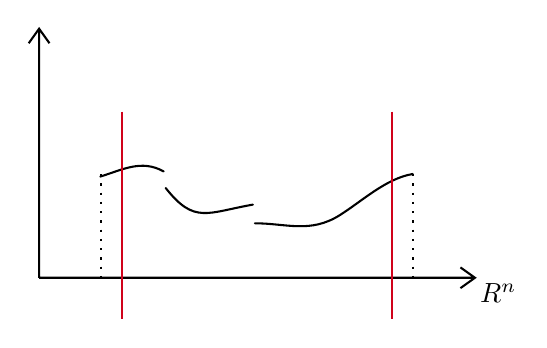
\begin{tikzpicture}[x=0.75pt,y=0.75pt,yscale=-1,xscale=1]
        %uncomment if require: \path (0,183); %set diagram left start at 0, and has height of 183

        %Shape: Axis 2D [id:dp8877340503666933] 
        \draw  (190,140) -- (400,140)(190,20) -- (190,140) -- cycle (393,135) -- (400,140) -- (393,145) (185,27) -- (190,20) -- (195,27)  ;
        %Curve Lines [id:da3663302699262805] 
        \draw [color={rgb, 255:red, 0; green, 0; blue, 0 }  ][line width=0.75] [line join = round][line cap = round]   (219.5,91.25) .. controls (230.51,87.81) and (239.41,82.87) .. (250,88.75) ;
        %Curve Lines [id:da43487324241444214] 
        \draw [color={rgb, 255:red, 0; green, 0; blue, 0 }  ][line width=0.75] [line join = round][line cap = round]   (251,96.75) .. controls (264.82,114.26) and (270.83,108.66) .. (293,104.75) ;
        %Curve Lines [id:da5404858145756182] 
        \draw [color={rgb, 255:red, 0; green, 0; blue, 0 }  ][line width=0.75] [line join = round][line cap = round]   (294,113.75) .. controls (309.1,113.75) and (320.69,118.82) .. (335,109.75) .. controls (345.89,102.84) and (357.28,92.12) .. (370,90) ;
        %Straight Lines [id:da4922719589175637] 
        \draw  [dash pattern={on 0.84pt off 2.51pt}]  (220,90) -- (220,140) ;
        %Straight Lines [id:da972371294781222] 
        \draw  [dash pattern={on 0.84pt off 2.51pt}]  (370,90) -- (370,140) ;
        %Straight Lines [id:da07765020824369273] 
        \draw [color={rgb, 255:red, 208; green, 2; blue, 27 }  ,draw opacity=1 ]   (230,60) -- (230,160) ;
        %Straight Lines [id:da3369737599733198] 
        \draw [color={rgb, 255:red, 208; green, 2; blue, 27 }  ,draw opacity=1 ]   (360,60) -- (360,160) ;

        % Text Node
        \draw (401,141.4) node [anchor=north west][inner sep=0.75pt]    {$\mathbb{R}^{n}$};

    \end{tikzpicture}
\end{figure}
\FloatBarrier

Il vero problema è il supporto compatto. La funzione di $L^{2}$ è tipicamente diversa da $0$ fino al bordo. Dobbiamo pensare che la funzione sia estesa a $0$ fuori per poter fare la media in prossimità del bordo. La fregatura è ci troviamo con delle cose ben diverse da $0$, anche fuori dal bordo.

Come si ottiene il supporto compatto? Si segano via preventivamente le parti finali, moltiplicando per una funzione indicatrice. La parte di norma che perdiamo è trascurabile in $L^{2}$.

Se lo facciamo in $H^{1}$ \textbf{non ci basta misurare quello che perdiamo nella funzione}, ma \textbf{anche quello che perdiamo nella derivata}. E questo ci impedisce di fare il gioco.

Se prendiamo la Heaviside \textit{rattoppata} la norma delle funzioni che perdiamo è poca, ma la norma delle derivate delle funzioni esplode.

Si può dimostrare che
\begin{equation*}
    u\in H^{1}(\Omega) \cap C(\overline{\Omega }) \ \ \Rightarrow \ \ \left\{u\in H^{1}_{0}(\Omega) \ \ \Leftrightarrow \ \ u_{|\partial \Omega } =0\right\}
\end{equation*}
In poche parole non possiamo dire davvero che una funzione fa $0$ al bordo, ma possiamo dire se è o non è approssimabile da funzioni a supporto compatto; e se lo è, moralmente è come se facesse $0$ al bordo.

Quindi $H^{1}_{0}(\Omega)$ è un sottospazio chiuso di $H^{1}(\Omega)$.

\subsection{Disuguaglianza di Poincaré}
\begin{theorem}
    [Disuguaglianza di Poincaré] Sia $\Omega \subset \mathbb{R}^{n}$ un dominio \textbf{limitato}. Allora $\exists C_{P}  >0$ (costante di Poincaré) tale che
    \begin{equation}
        \Vert u\Vert _{L^{2}(\Omega)} \leqslant C_{P}\Vert \nabla u\Vert _{L^{2}(\Omega)} ,\ \ \forall u\in H^{1}_{0}(\Omega)
    \end{equation}
\end{theorem}
A priori per controllare le funzioni di $H^{1}$ bisogna controllare loro e le loro derivate\footnote{Funzione che oscilla moltissimo, ma di valori bassi, e funzione costante a valore altissimo, sono due esempi estremi in cui vediamo che è necessario controllarle entrambe.}. In $H^{1}_{0}$ \textbf{la funzione è sempre controllata dalla derivata.}
\begin{oss}
    Un'immediata conseguenza è che l'unica costante che può appartenere ad $H^{1}_{0}$ è la costante nulla, ulteriore indice che \textit{ci stanno le cose che si annullano al bordo.}

    Ovvero, se consideriamo un dominio limitato $(|\Omega |< +\infty)$, le costanti stanno in $H^{1} $: $u(x) \equiv c,u\in H^{1}(\Omega)$,  ma
    \begin{equation*}
        u\in H_{0}^{1}(\Omega) \ \ \Leftrightarrow \ \ c=0
    \end{equation*}
\end{oss}

\LezioneV{08/04/2021}
\begin{oss}
    La disuguaglianza di Poincaré non vale in $H^{1} $ proprio perché ci basta prendere una costante dove otterremmo la sua norma $L^2$, generalmente maggiore di zero, maggiorata da $0$.
\end{oss}
\begin{dimostrazione}
    Si svolge in due passi. Sfruttiamo il fatto che $\mathcal{D}(\Omega)$ è denso in $H_{0}^{1}(\Omega)$:
    \begin{enumerate}
        \item dimostro la Disuguaglianza di Poincaré in $\mathcal{D}(\Omega)$,
        \item per approssimazione estendo ad $H_{0}^{1}(\Omega)$.
    \end{enumerate}

    \textbf{Passo 1.}

    Fisso una funzione test $\varphi \in \mathcal{D}(\Omega)$ e costruisco un apposito campo vettoriale $\boxed{\mathbf{F}(\x) =\varphi ^{2}(\x)\x}$ su cui applicare il teorema della divergenza
    \begin{equation*}
        \int _{\Omega }\mathrm{div}\mathbf{F} \dxx =\int _{\partial \Omega }\mathbf{F} \cdotp \bm{\nu } \dsig
    \end{equation*}
    Per applicare il teorema della divergenza devo controllare due cose:
    \begin{enumerate}
        \item Il campo deve essere di classe $C^{1}$ fino al bordo: in questo caso $\varphi $ è $C^{\infty }$ fino al bordo quindi non ho problemi.
        \item Il bordo del dominio deve essere sufficientemente regolare, ad esempio Lipschitziano (in modo tale che la normale sia definita quasi ovunque). Non ho alcuna ipotesi però sul dominio $\Omega $ nel teorema: so solo che $\varphi $ è a supporto compatto, eventualmente molto brutto, contenuto in $\Omega $ \textit{limitato}, allora esiste una palla (centrata nell'origine, ma non importa) che contiene $\Omega $
              \begin{equation*}
                  B_{M}(\zer) \supset \Omega
              \end{equation*}

              \begin{figure}[H]
                  \centering
                  \tikzset{every picture/.style={line width=0.75pt}} %set default line width to 0.75pt        

                  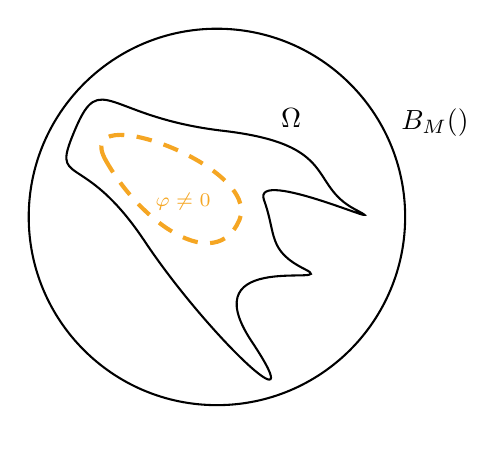
\begin{tikzpicture}[x=0.75pt,y=0.75pt,yscale=-1,xscale=1]
                      %uncomment if require: \path (0,206); %set diagram left start at 0, and has height of 206

                      %Shape: Ellipse [id:dp028463181051103792] 
                      \draw   (114.2,103.68) .. controls (114.2,53.6) and (154.8,13) .. (204.88,13) .. controls (254.97,13) and (295.57,53.6) .. (295.57,103.68) .. controls (295.57,153.77) and (254.97,194.37) .. (204.88,194.37) .. controls (154.8,194.37) and (114.2,153.77) .. (114.2,103.68) -- cycle ;
                      %Shape: Polygon Curved [id:ds6991047652266367] 
                      \draw   (136.62,61.43) .. controls (149,32.34) and (151.59,55.66) .. (207.86,62.19) .. controls (264.13,68.73) and (248.57,88.03) .. (271.52,100.09) .. controls (294.47,112.14) and (221.5,78.87) .. (227.56,95.54) .. controls (233.63,112.21) and (229.08,119.79) .. (247.27,128.88) .. controls (265.46,137.98) and (191.44,118.4) .. (221.75,163.87) .. controls (252.07,209.34) and (200.28,160.71) .. (169.97,115.24) .. controls (139.65,69.77) and (124.24,90.53) .. (136.62,61.43) -- cycle ;
                      %Shape: Polygon Curved [id:ds5733783657314724] 
                      \draw  [color={rgb, 255:red, 245; green, 166; blue, 35 }  ,draw opacity=1 ][dash pattern={on 5.63pt off 4.5pt}][line width=1.5]  (151.33,76.44) .. controls (133.97,45.72) and (227.01,79.22) .. (215.66,105.26) .. controls (204.3,131.31) and (168.69,107.15) .. (151.33,76.44) -- cycle ;

                      % Text Node
                      \draw (292.28,49.94) node [anchor=north west][inner sep=0.75pt]    {$B_{M}(\zer)$};
                      % Text Node
                      \draw (234.31,49.81) node [anchor=north west][inner sep=0.75pt]    {$\Omega $};
                      % Text Node
                      \draw (173.72,90.86) node [anchor=north west][inner sep=0.75pt]  [font=\scriptsize,color={rgb, 255:red, 245; green, 166; blue, 35 }  ,opacity=1 ]  {$\varphi \neq 0$};


                  \end{tikzpicture}
              \end{figure}
              \FloatBarrier


              allora $\varphi \in \mathcal{D}(B_{M}(\zer))$ (basta estenderla a $0$ fuori) e posso applicare il teorema della divergenza direttamente su $B_{M}(\zer)$.
    \end{enumerate}

    Ma allora essendo $\varphi $ a supporto compatto anche il campo è supporto compatto e si annulla sul bordo:
    \begin{equation}
        \int _{\Omega }\mathrm{div}\mathbf{F} \dxx =\underbrace{\int _{\partial \Omega }\mathbf{F} \cdotp \bm{\nu }\dsig }_{=0} =0
        \label{eq:af-dim-poincare}
    \end{equation}
    Ricordiamo la formula di derivazione di Leibniz:
    \begin{equation*}
        \mathrm{div}(f\mathbf{G}) =\nabla f\cdotp \mathbf{G} +f\mathrm{div}\mathbf{G} .
    \end{equation*}
    Posso modificare la \eqref{eq:af-dim-poincare}:
    \begin{align*}
        0 & =\int _{\Omega }\mathrm{div}\mathbf{F} \dxx =\int _{\Omega }\mathrm{div}\left(\varphi ^{2}(\x)\x\right) \dxx                                                      \\
          & =\int _{\Omega }\big[\underbrace{2\varphi \nabla \varphi }_{\nabla \left(\varphi ^{2}\right)} \cdotp \x +\varphi ^{2}\underbrace{\mathrm{div}\x}_{=n}\big] \dxx ,
    \end{align*}
    cioè, usando Cauchy-Schwarz:
    \begin{align*}
        n\int _{\Omega } \varphi ^{2} \dxx =-2\int _{\Omega } \varphi \nabla \varphi \cdotp \x \dxx & \leqslant 2\left| \int _{\Omega } \varphi \nabla \varphi \cdotp \x \dxx\right| \\
                                                                                                    & \leqslant 2\int _{\Omega }| \varphi | | \nabla \varphi | | \x| \dxx ,
    \end{align*}
    per ipotesi, se il dominio è limitato, $\displaystyle \Omega \subset B_{M}(\zer)$, per cui se $\displaystyle \x \in \Omega $ allora il suo modulo è maggiorato da una certa costante $\displaystyle | \x| \leqslant M$. Infine per Cauchy-Schwarz:
    \begin{align*}
        n\int _{\Omega } \varphi ^{2} \dxx & \leqslant 2M\int _{\Omega }| \varphi | | \nabla \varphi | \dxx                                                         \\
                                           & \leqslant 2M\left(\int _{\Omega } \varphi ^{2}\right)^{1/2}\left(\int _{\Omega }| \nabla \varphi | ^{2}\right)^{1/2} ,
    \end{align*}
    quindi semplificando una norma $\displaystyle L^{2}$ di $\displaystyle \varphi $ ottengo:
    \begin{equation*}
        \left(\int _{\Omega } \varphi ^{2} \dxx\right)^{1/2} \leqslant \underbrace{\frac{2M}{n}}_{C_{P}}\left(\int _{\Omega }| \nabla \varphi | ^{2}\right)^{1/2} .
    \end{equation*}
    \textbf{Passo 2.}

    Per il passo 1 so che
    \begin{equation*}
        \exists \ C_{P} :\ \Vert \varphi \Vert _{L^{2}} \leqslant C_{P}\Vert \nabla \varphi \Vert _{L^{2}} ,\ \ \forall \varphi \in \mathcal{D}(\Omega) .
    \end{equation*}
    Ma per inclusione densa:
    \begin{equation*}
        u\in H_{0}^{1}(\Omega) \ \ \Leftrightarrow \ \ \varphi _{n}\xrightarrow{L^{2}} u,\ \nabla \varphi _{n}\xrightarrow{L^{2}} \nabla u,
    \end{equation*}
    allora per continuità della norma, facendo il limite ottengo
    \begin{gather*}
        \Vert \varphi _{n}\Vert _{L^{2}} \leqslant C_{P}\Vert \nabla \varphi _{n}\Vert _{L^{2}}\\
        \downarrow \\
        \Vert u\Vert _{L^{2}} \leqslant C_{P}\Vert \nabla u\Vert _{L^{2}}
    \end{gather*}
\end{dimostrazione}
Si noti che in realtà\footnote{e questa è una chicca per l'orale.} per ipotesi serve che $\Omega$ sia limitato almeno in una direzione, ma non per forza tutte. Quando costruiamo il campo ausiliario, è sufficiente scegliere un $\x$ tale che abbia componenti nulle direzioni illimitate e $x_{i}$ nella $i$-esima direzione in cui è limitato. I calcoli si svolgono analogamente. Attenzione che in quel caso la divergenza di $\x$ non è più $n$, ma $1,2, \cdots $ a seconda del caso. Si noti che la stima \emph{peggiora} dato che non dividiamo per $n$, ma per qualcosa di più piccolo.
\begin{oss}
    Con la dimostrazione ho trovato anche una stima della costante $\displaystyle C_{P}$:
    \begin{equation*}
        C_{P} =\frac{2M}{n} .
    \end{equation*}
    Tuttavia non è la migliore costante possibile. Quest'ultima si trova pensando a:
    \begin{equation*}
        \Vert u\Vert _{L^{2}}^{2} \leqslant C_{P}^{2}\Vert \nabla u\Vert _{L^{2}}^{2}
    \end{equation*}
    che è equivalente a dire che
    \begin{equation*}
        \frac{1}{C_{P}^{2}} \leqslant \frac{\Vert \nabla u\Vert _{L^{2}}^{2}}{\Vert u\Vert _{L^{2}}^{2}} ,
    \end{equation*}
    la migliore costante si trova per il valore che minimizza $\displaystyle C_{P}$, cioè che massimizza $\displaystyle 1/C_{P}^{2}$, cioè che minimizza il secondo termine:
    \begin{equation}
        \frac{1}{C_{P}^{2}} =\lambda _{1}(\Omega) =\min_{u\in H_{0}^{1}(\Omega) ,\ u\neq 0}\frac{\int _{\Omega }| \nabla u| ^{2}}{\int _{\Omega } u^{2}}
    \end{equation}
    $\displaystyle \lambda _{1}$ è il primo autovalore di $\displaystyle -\Delta $ con condizione di Dirichlet e assume significati fisici importanti:
    \begin{itemize}
        \item la frequenza di base di vibrazione di $\displaystyle \Omega $,
        \item è legato alla \textit{sopravvivenza} in fenomenti di reazione-diffusione.
    \end{itemize}
\end{oss}
\begin{oss}
    In generale:
    \begin{equation*}
        \textcolor[rgb]{0.25,0.46,0.02}{\Vert u\Vert _{H^{1}(\Omega)}^{2}} =\Vert u\Vert _{L^{2}(\Omega)}^{2} +\textcolor[rgb]{0.82,0.01,0.11}{\Vert \nabla u\Vert _{L^{2}(\Omega)}^{2}}
    \end{equation*}
    Se $\displaystyle u\in H_{0}^{1}(\Omega)$, grazie a Poincaré
    \begin{equation}
        \textcolor[rgb]{0.82,0.01,0.11}{\Vert \nabla u\Vert _{L^{2}(\Omega)}^{2}} \leqslant \underbrace{\Vert u\Vert _{L^{2}(\Omega)}^{2} +\textcolor[rgb]{0.82,0.01,0.11}{\Vert \nabla u\Vert _{L^{2}(\Omega)}^{2}}}_{\textcolor[rgb]{0.25,0.46,0.02}{\Vert u\Vert _{H^{1}(\Omega)}^{2}}} \leqslant \left(C_{P}^{2} +1\right)\textcolor[rgb]{0.82,0.01,0.11}{\Vert \nabla u\Vert _{L^{2}(\Omega)}^{2}}
        \label{eq:af-stima-poincare}
    \end{equation}
    Quindi in $\displaystyle H_{0}^{1}$ (che ricordiamo è spazio di Hilbert essenso sottospazio chiuso di uno spazio di Hilbert) ci sono due norme equivalenti\footnote{Ce ne sono tante, ma ne abbiamo messe in evidenza due.}:
    \begin{equation*}
        \Vert u\Vert _{H^{1}(\Omega)} \ \ \ \ \ \ \Vert \nabla u\Vert _{L^{2}(\Omega)}
    \end{equation*}
\end{oss}
A seconda che si preferisca un'analisi numerica o teorica si usano, rispettavemente, la prima o la seconda norma.